\documentclass{beamer}
\usepackage{HECbeamer}
\usepackage{icomma}

\title[\color{white}{MATH 60604 \S~5a - Introduction aux données corrélées et longitudinales}]{\texorpdfstring{MATH 60604 \\Modélisation statistique \\ \S~5a - Introduction aux données corrélées et longitudinales}{MATH 60604 \\Modélisation statistique \\ \S~5a - Introduction aux données corrélées et longitudinales}}
\author{}
\institute{HEC Montréal\\
Département de sciences de la décision}
\date{} 

\begin{document}
\frame{\titlepage}

\begin{frame}
\frametitle{Modifications du modèle de régression linéaire ordinaire}
\bi 
\item Le but de ce chapitre est de voir comment prendre en compte la dépendance entre observations.
\item On se cantonne à la modélisation de la matrice de covariance pour prendre en compte la dépendance entre observations (pour les données longitudinales et groupées) et l'hétéroscédasticité de groupe.
\ei
\end{frame}
\begin{frame}
\frametitle{Quand les données ne sont pas indépendantes}
\begin{itemize}
\item Si les observations sont positivement corrélées, les erreurs-type estimés sont \textbf{trop petites}.
\item On détecte des différences significatives qui ne le sont pas en réalité (erreur de type I enflée, ou faux positifs plus fréquents).
\end{itemize}
\end{frame}
\begin{frame}
\frametitle{Sources de corrélation}
Généralement, la corrélation entre observations provient de
\bi
\item  dépendance temporelle, catégorisée en
\bi 
\item données longitudinales: mesures répétées sur des individus (séries courtes)
\item séries chronologiques: observations à plusieurs périodes (séries longues). Ces données nécessitent des modèles adaptés qui ne sont pas couverts dans ce cours.
\ei 
\item  données groupées: données sur des sujets qui ne sont pas indépendants (familles, groupes, etc.)
\ei
\end{frame}
\begin{frame}
\frametitle{Moments de vecteurs aléatoires}
\bi
\item Soit un vecteur aléatoire $\bs{Y}$ de dimension $n$. 
\bi
\item Dans la situation qui nous intéresse, un tel vecteur sera habituellement
composé des mesures répétées sur un individu ou bien d'observations d'un
groupe d'individus. 
\ei
\item L'espérance (ou moyenne théorique) d'un tel vecteur est $\E{\bs{Y}}$ calculée terme par terme, $\E{\bs{Y}} = (\E{Y_1}, \ldots, \E{Y_n})$.
\item On note aussi la variance de la $i$e composante $\sigma_{ii} = \sigma^2_i=\Va{Y_i}$.
\item De même, la covariance entre la $i$e et la $j$e composante est  $\sigma_{ij}=\Co{Y_i, Y_j}$.
\ei
\end{frame}

\begin{frame}
\frametitle{Matrice de covariance}
 Pour un vecteur aléatoire $\bs{Y}$, 
on définit la \alert{matrice de covariance} comme étant la matrice symétrique $n\times n$
\[
\Co{\bs{Y}}=
  \begin{pmatrix}
    \sigma_{1}^2 & \sigma_{12} & \sigma_{13} & \cdots & \sigma_{1n} \\
     \sigma_{21} & \sigma_{2}^2 & \sigma_{23} & \cdots & \sigma_{2n} \\
      \sigma_{31} & \sigma_{32} & \sigma_{3}^2 & \ddots & \sigma_{3n} \\
    \vdots &  \vdots &  \ddots & \ddots &  \vdots \\
        \sigma_{n1} & \sigma_{n2} & \sigma_{n3} & \cdots & \sigma_{n}^2 \\
  \end{pmatrix}.
\]
\bi
\item Le $i$e élément de la diagonale de  $\Co{\bs{Y}}$ est la variance de $Y_i$.
\item Cette matrice est symmétrique, avec  $\sigma_{ij}=\sigma_{ji}$.
\ei
\end{frame}

\begin{frame}
\frametitle{Matrice de corrélation}
\bi
\item La corrélation entre $Y_i$ et $Y_j$ est donnée par:
\begin{align*}
\rho_{ij}=\Cor{Y_i, Y_j}=\frac{\sigma_{ij}}{\sigma_i\sigma_j}.
\end{align*}
\item La \alert{matrice de corrélation} de $\bs{Y}$ est définie comme étant la matrice symétrique
$n\times n$ qui contient un sur la diagonale et les corrélations hors diagonale, 
\[
\Cor{\bs{Y}}=
  \begin{pmatrix}
    1 & \rho_{12} & \rho_{13} & \cdots & \rho_{1n} \\
     \rho_{21} & 1 & \rho_{23}& \cdots & \rho_{2n} \\
     \rho_{31} & \rho_{32} & 1& \ddots & \rho_{3n} \\
    \vdots &  \vdots &  \ddots & \ddots &  \vdots \\
        \rho_{n1} & \rho_{n2} & \rho_{n3} & \cdots & 1 \\
  \end{pmatrix}.
\]
\ei
\end{frame}
\begin{frame}
 \frametitle{Modélisation de la covariance entre observations}
 Un des traits principaux des données
corrélées et longitudinales est la nécessité de tenir compte de la corrélation
intra-classe.
\bi \item cela reviendra souvent à modéliser la matrice de covariance
des observations d'un même groupe (ou d'un même individu dans le cas de
mesures répétées).
\ei
\end{frame}

\begin{frame}[fragile]
\frametitle{Études longitudinales sur des sujets indépendants}
\bi
\item Das ce type d'études, plusieurs mesures (habituellement à différents moments dans le temps) sont prises sur les mêmes individus. 
\bi

\item on nomme ces données \alert{mesures répétées} ou \alert{données longitudinales}; les économètres parlent plutôt de \alert{données de panel}.
\ei
\item Les individus sont \alert{indépendants} les uns des autres, mais les mesures pour un même sujet ne sont pas indépendantes.
\item Un fichier de données pour de telles études a typiquement ce format:
\ei
{\footnotesize 
\begin{table}
\centering

\begin{tabular}{cccc}
 \toprule 
 \textbf{sujet} & \textbf{temps} & \textbf{score} & \textbf{sexe}\\
 \midrule 
 1 & 1 & 5 & 0 \\
 1 & 2 & 6 & 0 \\
 1 & 3 & 4 & 0 \\
 2 & 1 & 2 & 1 \\
 2 & 2 & 4 & 1 \\
 2 & 3 & 7 & 1 \\
 \bottomrule
\end{tabular}
\end{table}
}

\end{frame}

\begin{frame}
\frametitle{Études sur des sujets non indépendants}
\bi
\item Dans ce type d'étude, les sujets sont échantillonnés à l'intérieur d'un \alert{groupe}.
\item Voici plusieurs exemples:
\bi

\item sujets échantillonnés dans plusieurs ménages (familles), 
\item sujets échantillonnés dans plusieurs entreprises, 
\item sujets échantillonnées dans des écoles, dans des hôpitaux, etc.
\ei
\item Dans tous ces cas, il y a de la corrélation entre les mesures des sujets appartenant au même groupe (famille, école, entreprise).
\ei
\end{frame}

\begin{frame}
\frametitle{Les données corrélées sont des données groupées}
\bi
\item On peut toujours considérer les données corrélées comme étant des données groupées avec de la corrélation intra-groupe.
\item Dans le cas de données longitudinales, le groupe est le sujet lui-même et on a donc plusieurs observations par groupe.
\item Dans les autres cas, les groupes sont les ménages, les écoles, les hôpitaux, les entreprises, etc.
\ei
\begin{center}
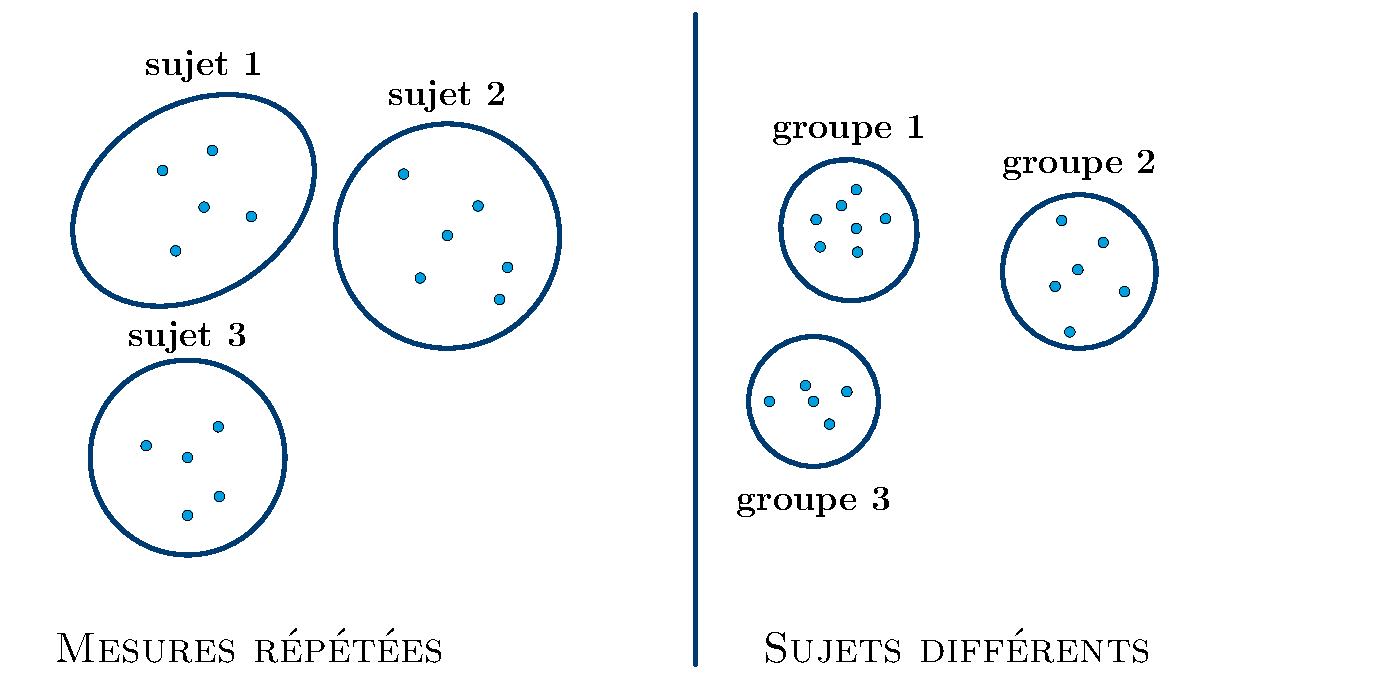
\includegraphics[width = 0.8\linewidth]{img/c5/06-correlated-groups_fr.pdf}
\end{center}
Dans tous les cas, un point égale une ligne du fichier de données.
\end{frame} 


\begin{frame}
\frametitle{Que se passe-t-il si on ignore la corrélation intra-groupes?}
\bi
\item Supposons que nous avons des données groupées et que nous voulons faire un test-$t$ pour un échantillon sur ces données à niveau 5\%.
\item La figure suivante montre quelle est la vraie probabilité d'erreur
de type I (qu'on pense être de 5\%) en fonction de la corrélation intra-groupe
pour différentes valeurs de la taille des groupes $m$. 
\begin{center}
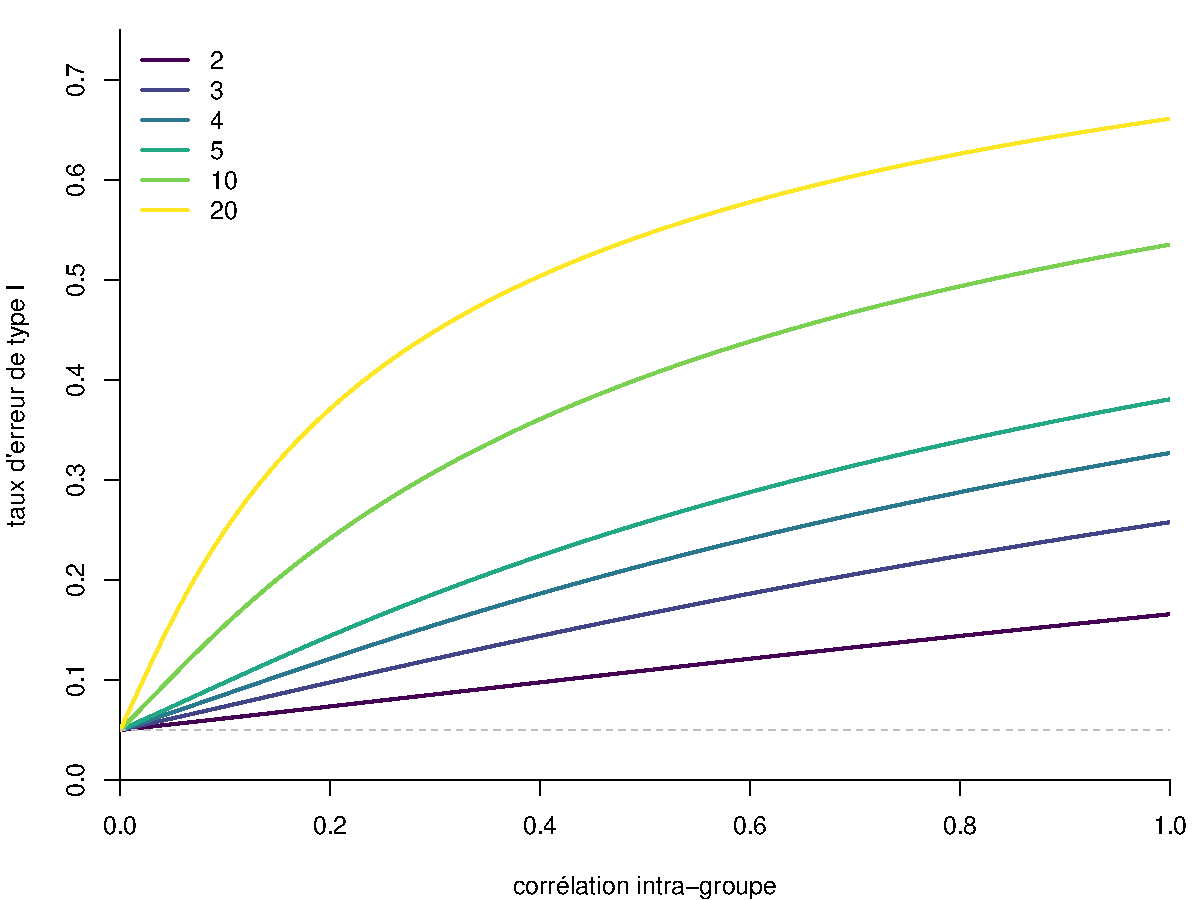
\includegraphics[width = 0.65\linewidth]{img/c5/06-correlated-typeIerrorinf_fr.pdf}
\end{center}
\ei
\end{frame}
 
\begin{frame}
\frametitle{Inflation de l'erreur de type I pour les données corrélées}
\bi
\item Il est frappant de voir à quel point la probabilité
d'erreur de type I augmente rapidement avec la corrélation et qu'elle augmente
d'autant plus vite que le nombre d'observations par groupe est grand. 
\item La
conclusion tirée du test-$t$ n'est pas valide si on ne tient pas compte de la
corrélation intra-groupe.
\item La distortion du niveau illustre que l'inférence statistique n'est généralement
plus valide lorsqu'elle découle d'une méthode supposant l'indépendance entre
les observations et que ce n'est pas vérifiée.
\ei
\end{frame}

\end{document}
